\documentclass[a4paper,11pt,notitlepage]{article}
\usepackage{sprawozdanie-ato}

\begin{document}


\title{\
Laboratorium Sieci Komputerowych\\\
Konfiguracja łącz i interfejsów sieciowych\
}
\author{\
Tomasz Cudziło, Barnaba Turek\\
\textsc{PW EE Informatyka}\\[6pt]
}
\date{\today}

\maketitle
\tableofcontents


\section{Cel ćwiczenia}

W ramach laboratorium mieliśmy za zadanie własnoręcznie skonfigurować i
przetestować kilka interfejsów sieciowych w systemie \bsd. Spośród dostępnych
łącz postanowiliśmy przetestować:

\begin{description}
    \item[łącze przewodowe \eth\textnormal{,}] które było dostępne na naszej
    stacji roboczej i podłączone fizycznie do sieci laboratorium, jednak nie
    było skonfigurowane na maszynie.
    \item[łącze radiowe \wifi\textnormal{,}] w ramach testowania którego,
    wypróbowaliśmy dwa tryby pracy: połączenie typu \emph{punkt-punkt (P2P)},
    oraz połączenie do~\emph{punktu dostępowego (AP)}.
    \item[łącze radiowe \bt\textnormal{,}] dla którego połączyliśmy dwie
    maszyny laboratoryjne w układzie klient\dywiz serwer.
    \item[łącze szeregowe \uart\textnormal{,}] poprzez które połączyliśmy się
    z~konsolą maszyny \zielone{} za pomocą kabla szeregowego.
\end{description}


\section{Istniejąca konfiguracja stanowiska}


\section{Wykonanie ćwiczenia}
\section{bluetooth}
\label{sec:bt}
\subsection{Wprowadzenie}
Bluetooth to własnościowy standard komunikacji bezprzewodowej.

Korzystając z~połączenia Bluetooth możliwe jest tworzenie sieci \texttt{PAN} - Personal Area Network.

Sieci \texttt{PAN} oparte o~bluetooth pozwalają na połączenie maksymalnie 8 urządzeń w~konfiguracji klienci\dywiz serwer\cite{wiki:pan}.
W~sieci występuje jeden serwer i~wszyscy klienci powinni znajdować się w~jego zasięgu.

Możliwe jest także zwiększenie zasięgu sieci poprzez węzły pośrednie (tzw. \emph{scatternet})\cite{bt}.
\begin{figure}[h]
  \centering
  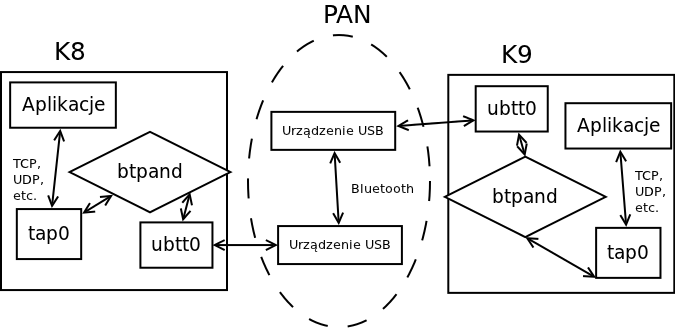
\includegraphics[width=\textwidth]{figury/schemat-bluetooth.png}
  \caption{Schemat ideowy}
\end{figure}

W systemie FreeBSD na którym mamy zajęcia połączenia w tej technologii można realizować za pomocą wirtualnego urządzenia \texttt{TAP}, na które demon \texttt{btpand} przekierowuje pakiety.

\subsection{Przebieg ćwiczenia}
Po zalogowaniu się na maszynę laboratoryjną załadowaliśmy niezbędne sterowniki (zgodnie z~instrukcjami podanymi przez skrypt \texttt{sterowniki -b}: \texttt{uhci, ehci, ng\_ubt}.
Są to sterowniki odpowiedzialne za stos \texttt{USB} oraz samo urządzenie bluetooth (podłączone do komputera przez \texttt{USB}).

Po załadowaniu sterowników musieliśmy odłączyć i~podłączyć urządzenie, żeby zostało wykryte.

\begin{lstlisting}[caption={Sprawdzenie, że urządzenie zostało wykryte}]
$ dmesg | tail
ugen4.2: <ZyDAS> at usbus4
ugen1.2: <Logitech> at usbus1
ugen0.2: <vendor 0x0a12> at usbus0^
ubt0: <vendor 0x0a12 product 0x0001, class 224/1, rev 1.10/3.73, addr 2> on usbus0
\end{lstlisting}

Kiedy upewniliśmy się, ze urządzenie zostało poprawnie rozpoznane, zgodnie z~instrukcją uruchomiliśmy usługę \texttt{bluetooth}.
\begin{lstlisting}[caption={Sprawdzenie, że urządzenie zostało wykryte}]
$ sudo service bluetooth onestart ubt0
\end{lstlisting}
Polecenie to nie uruchamia żadnego systemowego demona, ale konfiguruje urządzenie bluetooth do pracy, za pomocą komend \texttt{ngctl} i~\texttt{hccontrol}.

Polecenie \texttt{ngctl} służy do tworzenia i~wysyłania komand do węzła \emph{netgraph}.
\emph{Netgraph} to podsystem jądra, który pozwala obsługiwać różne interfejsy (L2TP, PPTP, ATM, bluetooth). Pozwala modularnie implementować protokoły (niezależnie od urządzeń) i~zapewnia spójny system komend dla różnych protokłów i~urządzeń\cite{man:netgraph}.

Polecenie \texttt{hccontroll} zapewnia obsługę komend specyficznych dla interfejsów \emph{Bluetooth}.

Następnie połączyliśmy się za pomocą bluetooth z~maszyną \textbf{k8}:
\begin{lstlisting}[caption={Połączenie na poziomie protokołu bluetooth}]
$ hccontrol read_bd_addr #k8
BD_ADDR: 00:08:1b:00:d3:3a

# adresy urzadzen beda potrzebne do zestawienia sieci PAN
# i pozwalaja sprawdzicz, czy urzadzenie zostalo poprawnie zainicjowane
# w podsystemie netgraph.

$ hccontrol read_bd_addr #k9
BD_ADDR: 00:08:1b:00:2e:e3

# sprawdzamy, czy 'widzimy' docelowe urzadzenie

$ sudo hccontrol inquiry
[...]
Inquiry result, num_responses=1
Inquiry result #0
  BD_ADDR: F4
  Page Scan Rep. Mode: 0x1
  Page Scan Period Mode: 0x2
  Page Scan Mode: 00
  Class: 00:1f:00
  Clock offset: 0x66c4
[...]
Inquiry complete. Status: No error [00]

# sprawdzamy czy mozemy sie z nim komunikowac

$ l2ping -a 00:08:1b:00:d3:3a
44 bytes from K8 seq_no=1 time=26.587 ms result=0
44 bytes from K8 seq_no=2 time=22.212 ms result=0
44 bytes from K8 seq_no=3 time=29.836 ms result=0
44 bytes from K8 seq_no=4 time=39.968 ms result=0
44 bytes from K8 seq_no=5 time=20.572 ms result=0

# tworzymy siec pan (skrypt bt-pan uruchamia demona btpand)

$ sudo bt-pan -c 00:08:1b:00:d3:3a # utworzenie sieci pan z k8 w roli serwera

BD_ADDR: 00:08:1b:00:2e:e3
00:08:1b:00:2e:e3Starting sdpd.
btpand[1429]: Searching for NAP service at 00:08:1b:00:d3:3a
btpand[1429]: Found PSM 15 for service NAP
btpand[1429]: Opening connection to service 0x1116 at 00:08:1b:00:d3:3a
btpand[1429]: channel_open: (fd#4)
btpand[1429]: Using interface tap0 with addr 00:00:1b:00:2e:e3
btpand[1429]: channel_open: (fd#5)
skonfiguruj teraz interfejs tap0   np. ifconfig tap0 10.9
\end{lstlisting}

Skrypt bt-pan nie tylko połączył nas z urządzeniem bluetooth komputera \textbf{k8}, ale też utworzył wirtualny interfejs sieciowy.
Stworzony przez ten skrypt interfejs jest powiazany z konkretną siecią PAN.

Demon \texttt{btpand} opakowuje wychodzące pakiety wyższych warstw modelu OSI w~ramki protokołu Bluetooth Network Encapsulation Protocol (BNEP).
Protokół BNEP wspiera te same protokoły sieciowe, które wspiera IEEE 802.3/Ethernet\cite[bnep].

Demon \texttt{btpand} zapewnia przekierowanie pakietów \emph{ethernetowych} przychodzących na urządzenie Bluetooth na wirtualny interfejs (w~naszym przypadku \texttt{tap0}).

Uruchomił także demona \emph{sdpd}, który pozwala udostępniać usługi za pomocą bluetooth i~wyszukiwać usługi na innych urządzeniach.

Następnym krokiem było, zgodnie z~instrukcjami polecenia skryptu \texttt{bt-pan} skonfigurowaniu interfejsu tap0.
(A~także wykonanie analogicznych poleceń na maszynie k8).

\begin{lstlisting}[caption={Skonfigurowanie interfejsów zgodnie z~protokołem IP}]
$ sudo ifconfig tap0 10.8
$ ifconfig

[...]

tap0: flags=8843<UP,BROADCAST,RUNNING,SIMPLEX,MULTICAST> metric 0 mtu 1500
  options=80000<LINKSTATE>
  ether 00:08:1b:00:2e:e3
  inet 10.0.0.9 netmask 255.0.0.0 broadcast 10.255.255.255
  Opened by PID 1429

$ ping 10.8

64 bytes from 10.0.0.8: icmp_seq=0 ttl=64 time=68.957 ms
[...]

# wygenerowalismy ruch TCP na interfejsach korzystajac z polecenia netcat

$ sudo tcpdump -i tap0 host 10.8 tcp
tcpdump: verbose output suppressed, use -v or -vv for full protocol decode
listening on tap0, link-type EN10MB (Ethernet), capture size 65535 bytes
17:02:34.236847 IP 10.0.0.8.11342 > 10.0.0.9.1337: Flags [P.], seq 982177280:982177281, ack 3979280866, win 1040, options [nop,nop,TS val 13104042 ecr 1310253008], length 1
17:02:34.336347 IP 10.0.0.9.1337 > 10.0.0.8.11342: Flags [.], ack 1, win 1040, options [nop,nop,TS val 1310280520 ecr 13104042], length 0
17:02:34.777801 IP 10.0.0.8.11342 > 10.0.0.9.1337: Flags [P.], seq 1:2, ack 1, win 1040, options [nop,nop,TS val 13104579 ecr 1310280520], length 1
17:02:34.877216 IP 10.0.0.9.1337 > 10.0.0.8.11342: Flags [.], ack 2, win 1040, options [nop,nop,TS val 1310281061 ecr 13104579], length 0

\end{lstlisting}


\subsection{Połączenie szeregowe}

\subsubsection{Wprowadzenie}

Systemy z~rodziny *NIX pozwalają na korzystanie z~konsoli za pośrednictwem portu
szeregowego (zwykle rs\dywiz 232). Funkcja ta jest przydatna zarówno dla
administratorów (ponieważ nie trzeba podłączać klawiatury i~monitora do serwera)
jak i~programistów, pracujących nad sterownikami.

Skorzystaliśmy z~konsoli aby połączyć się z~urządzeniem \zielone{} z maszyny
\kdziew. Do zestawienia takiego połączenia za pomocą portu szeregowego potrzebny
jest kabel typu \emph{null\dywiz modem}\cite{serial-console}.

\subsubsection{Konfiguracja połączenia --- null\dywiz modem}
\label{sec:serial:null-modem}

Po załadowaniu niezbędnych sterowników i~podłączeniu kabla \emph{null\dywiz
modem} zajrzeliśmy do pliku \texttt{/etc/remote}, w~którym zdefiniowane są
systemy znane przez program \texttt{tip}.

Dla każdego systemu podana jest nazwa urządzenia oraz konfiguracja połączenia,
gdzie ustalane są m.in. typ kontroli parzystości i~prędkość transmisji.

\begin{lstlisting}[caption={\texttt{/etc/remote}}]
modem:dv=/dev/cuau0:br#115200:pa=none:
ps:dv=/dev/cuau0:br#115200:pa=none:
bt:dv=/dev/ttyp0:br#115200:pa=none:
\end{lstlisting}

Skorzystaliśmy z~urządzenia \texttt{ps}, ponieważ wynik polecenia
\texttt{sterowniki -s} sugerował, że mamy się połączyć z urządzeniem
\texttt{/dev/cuau0}. Do tego prędkość transmisji zgadzała się z zaproponowanymi
w wyjściu polecenia.

\begin{lstlisting}[caption={Połączenie z konsolą maszyny \zielone{} za pomocą programu \texttt{tip}.}]
k9% sudo tip ps
^Gconnected

Login incorrect
debian login:
debian login: +++RESET

POST: 012345689bcefghips1234ajklnopqr,,,tvwxy

comBIOS ver. 1.33c 20080626  Copyright (C) 2000-2008 Soekris Engineering.
\end{lstlisting}

Zastosowaliśmy polecenie z zestawu rozkazów Hayesa żeby zrestartować maszynę
\zielone{} i z pomocą prowadzącego uruchomiliśmy na niej system \bsd.

\subsubsection{Konfiguracja połączenia --- \bt}

Dzięki zastosowaniu modemu radiowego Firefly możliwe jest bezprzewodowe
połączenie z~konsolą. Modem Firefly posiada tryb pracy, w~którym w~przezroczysty
sposób zastępuje kabel szeregowy, jednak wymagane są dwa modemy na każde
połączenie.

Zamiast tego w~laboratorium każda z~maszyn Soekris ma podpięty jeden modem,
a~komputery\dywiz terminale łączą się z tym modemem za pomocą własnego,
niespecjalizowanego radia \bt. Rozwiązanie takie pozwala ograniczyć liczbę
potrzebnych modemów Firefly, wymaga jednak więcej konfiguracji.

Po załadowaniu niezbędnych sterowników i~wyszukaniu interesujących nas urządzeń
w~eterze (analogicznie do ćwiczenia \ref{sec:bt}), próbowaliśmy skorzystać ze
skryptu \texttt{bt-spp}. Niestety skrypt aktualnie nie zawsze daje oczekiwane
rezultaty.

Wykryliśmy, że problem dotyczy tworzenia nowego terminala przez polecenie
\texttt{rfcomm\_sppd}. Wyłączenie tej funkcjonalności ograniczyłoby zastosowania
skryptu \texttt{bt-spp}, ale na nasze potrzeby było wystarczające. Usunęliśmy ze
skryptu komendę tworzącą urządzenie pełniące rolę pseudo\dywiz terminala. W
efekcie konsola, z~którą chcemy się połączyć jest dostępna w~konsoli, z~której
się łączyliśmy, analogicznie do działania programu \texttt{tip} w~sekcji
\ref{sec:serial:null-modem}.

\begin{lstlisting}[caption={Połączenie z konsolą za pomocą programu \texttt{rfcomm\_sppd}.}]
# Na maszynie k9.
% hostname
k9

# Laczymy sie z maszyna Soekris poprzez modem Firefly.
% rfcomm_sppd -a F11
rfcomm_sppd[1656]: Starting on stdin/stdout...
Login:stud
Password:zetis

Last login: Fri Apr 13 04:57:21 on ttyu0
FreeBSD 9.0-STABLE (SOEKRIS) #0 r233366M: Sat Mar 24 00:57:52 CET 2012

# Jestesmy w konsoli maszyny Soekris.
so4801% hostname
so4801
\end{lstlisting}



\section{Wnioski i spostrzeżenia}


\end{document}
